% -*- fill-column: 80 -*-

\documentclass[11pt,a4paper]{article}

\usepackage[margin=2.5cm]{geometry}
\usepackage[dvipsnames]{xcolor}
\usepackage{todonotes}
\usepackage{microtype}
\usepackage{amssymb,amsmath}
\usepackage{mathpazo}
\usepackage{longtable,booktabs}
\usepackage{dcolumn}
\usepackage{graphicx}
\usepackage{natbib}
\usepackage{hyperref}
\usepackage[capitalise,noabbrev,nameinlink]{cleveref}
\hypersetup{
  pdftitle={Storing the Cardano ledger state on disk: analysis and design options},
  pdfborder={0 0 0},
  breaklinks=true
}
\usepackage{subcaption}
\usepackage{listings}

\begin{document}

\title{Ouroboros Leios simulation: \\
       building confidence in the performance results \\
       {\large \sc An IOHK technical report}
  }
\date{Version 1.0, April 2021}
\author{Andrea Vezzosi     \\ {\small \texttt{andrea@well-typed.com}} \\
   \and Wen Kokke          \\ {\small \texttt{wen@well-typed.com}} \\
   \and Duncan Coutts      \\ {\small \texttt{duncan@well-typed.com}}
   }

\maketitle

\section{Introduction}
\label{introduction}


\tableofcontents

\listoftodos

\section{Summary}
\label{summary}

\todo{List/name scenarios}
\section{Scenario 1}
\label{scenario1}
The least realistic scenario. Config:
\lstinputlisting[firstline=7]{scenario1/config.yaml}
\todo{remove config once scenario explained}

In Figure~\ref{fig:scenario1} we compute ideal times two ways:
\begin{itemize}
\item \textbf{ideal} -- Uses $3$ latencies for every communication.
\item \textbf{ideal-fitted} -- Uses $3$ latencies for RB and EB, but $4$ for IB and $3.5$ for Votes.
\end{itemize}
we see that ideal-fitted better matches the simulation.

The Relay mini-protocol involves the consumer first requesting new headers, so
it can take $4$ latencies to receive the body. When blocks are more sporadic,
like for EBs and RBs, the consumer has likely already sent a blocking request
for more headers, so $3$ latencies are enough.
Votes all get sent at the start of the slice, with default configuration at least, so we can expect consumers to reach the blocking stage again by the next burst. However, due to the large traffic, the $4$ latencies path likely sees some use too. This mix of behaviours can explain the better fit using $3.5$ latencies.
\todo{Compare with the more uniform voting pattern setting}

\begin{figure}[htbp]
    \centering
    \begin{subfigure}[b]{0.45\textwidth}
        \centering
        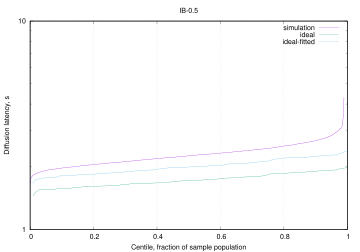
\includegraphics[width=\textwidth]{IB-0.5-vs-ideal-vs-fitted-fig.eps}
        \caption{IB diffusion to $0.50$ stake.}
        \label{scenario1:ib0.5}
    \end{subfigure}
    \hfill
    \begin{subfigure}[b]{0.45\textwidth}
        \centering
        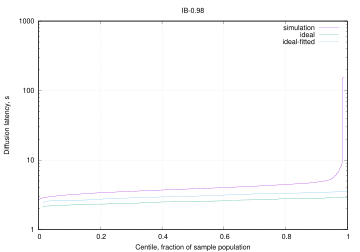
\includegraphics[width=\textwidth]{IB-0.98-vs-ideal-vs-fitted-fig.eps}
        \caption{IB diffusion to $0.98$ stake.}
        \label{scenario1:ib0.98}
    \end{subfigure}
    
    \vspace{1em}
    
    \begin{subfigure}[b]{0.45\textwidth}
        \centering
        \includegraphics[width=\textwidth]{EB-0.5-vs-ideal-vs-fitted-fig.eps}
        \caption{EB diffusion to $0.50$ stake.}
        \label{scenario1:eb0.5}
    \end{subfigure}
    \hfill
    \begin{subfigure}[b]{0.45\textwidth}
        \centering
        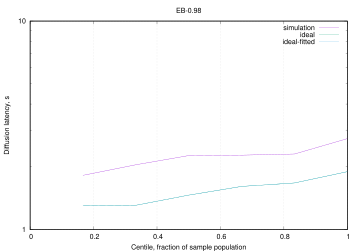
\includegraphics[width=\textwidth]{EB-0.98-vs-ideal-vs-fitted-fig.eps}
        \caption{EB diffusion to $0.98$ stake.}
        \label{scenario1:eb0.98}
    \end{subfigure}
    
    \vspace{1em}
    
    \begin{subfigure}[b]{0.45\textwidth}
        \centering
        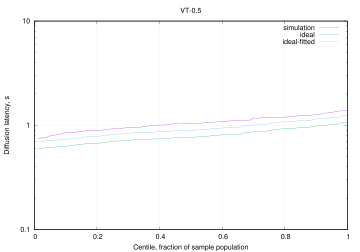
\includegraphics[width=\textwidth]{VT-0.5-vs-ideal-vs-fitted-fig.eps}
        \caption{VT diffusion to $0.50$ stake.}
        \label{scenario1:vt0.5}
    \end{subfigure}
    \hfill
    \begin{subfigure}[b]{0.45\textwidth}
        \centering
        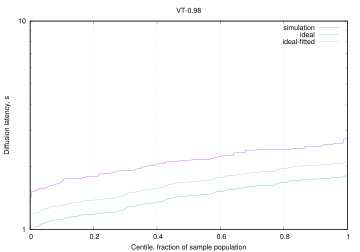
\includegraphics[width=\textwidth]{VT-0.98-vs-ideal-vs-fitted-fig.eps}
        \caption{VT diffusion to $0.98$ stake.}
        \label{scenario1:vt0.98}
    \end{subfigure}
    
    \vspace{1em}
    
    \begin{subfigure}[b]{0.45\textwidth}
        \centering
        \includegraphics[width=\textwidth]{RB-0.5-vs-ideal-vs-fitted-fig.eps}
        \caption{RB diffusion to $0.50$ stake.}
        \label{scenario1:rb0.5}
    \end{subfigure}
    \hfill
    \begin{subfigure}[b]{0.45\textwidth}
        \centering
        \includegraphics[width=\textwidth]{RB-0.98-vs-ideal-vs-fitted-fig.eps}
        \caption{RB diffusion to $0.98$ stake.}
        \label{scenario1:rb0.98}
    \end{subfigure}

    \caption{Scenario 1, diffusion latencies from slot start (300s run with default seed).}
    \label{fig:scenario1}
\end{figure}

\addcontentsline{toc}{section}{References}
\bibliographystyle{plainnat}
\bibliography{sim-realism}

\end{document}
